\chapter{Architektúra vrstvy Model}\label{architektura_model_vrstvy}

Model vrstva je štvrtou vrstvou MVVM(MV) architektúry. Táto vrstva je pre~zvyšné vrstvy zdrojom dát a~mechanizmov, ktoré~tieto dáta spracovávajú. Delí sa do~mnohých oblastí. Pre~komunikáciu s~týmito oblasťami sú vytvorení takzvaní \textit{manažéri}. Manažéri sú pristupovaný z~Model view vrstvy a~doručujú jej svoje služby, či~už informatívne alebo~výpočtové. Viac informácií o~vrstve Model je možné nájsť v~Podsekcii~\ref{model}.

Implementáciu Model vrstvy z~veľkej časti poznačila už spomínaná strata typovej informácie pri~komunikácii s~Model view vrstvou. Väčšina oblastí sa s~touto stratou vysporadúva podobným spôsobom:
\begin{itemize}
    \item \textbf{Komunikácia smerujúca z~vrstvy Model} - Pre~všetky dátové štruktúry, ktoré~sa využívajú mimo vrstvy Model, sú vytvorení predkovia, ktorí sú buďto negenerickí alebo~obsahujú kovariantné generické parametre. Tým pádom vedia byť prenášaní negenerickým spôsobom mimo vrstvy Model.
    \item \textbf{Komunikácia smerujúca do~vrstvy Model} - Pre~dátové štruktúry, ktorých typovú informáciu je potrebné v~Model vrstve opäť nadobudnúť, bol vytvorený tzv. \textit{Generic visitor pattern}. V~prípadoch, kedy nie je potrebné poznať ich presný typ, sa využíva klasické typové testovanie cez operátor \textit{is}.
\end{itemize} 

\textbf{Generic visitor pattern} je obdoba klasického návrhového vzoru \emph{Visitor pattern}. Pracuje na~podobnom princípe, kedy na~navštevovanej inštancii je volaná metóda \texttt{Visit} ktorej sa predá inštancia volajúcej triedy. Následne navštívená inštancia odpovie zavolaním metódy \texttt{Accept} na~dodanej volajúcej inštancii a~predaním samej seba v~argumente indikuje, ktorý~overload metódy \texttt{Accept} sa má zavolať.

V~prípade generic visitor pattern-u však volajúca trieda neimplementuje overload metódy \texttt{Accept} pre~každý možný typ navštevovanej inštancie ale~len jednu generickú metódu \texttt{Accept<T>}. V~typovom parametri \texttt{T} je následne predaná informácia o~type navštívenej inštancie.

\bigskip

V~následujúcich sekciách sa pozrieme detailnejšie na~aktuálne existujúce oblasti vrstvy Model a~ich vnútorné mechanizmy.

\section{Template-y}

Táto oblasť sa stará o~správu atribútových template-ov (len \textit{template-ov} pre~jednoduchosť). Viac informácií o~myšlienke a~funkcii template-ov je možné nájsť v~Podsekcii~\ref{templatey}. Čo do~obsahu je to jedna z~najmenších oblastí.  

Hlavným uzlom pre~komunikáciu z~Model view vrstvy je singleton trieda \texttt{TemplateManager}. Ten ponúka kolekciu všetkých template-ov, ktoré~je možné v~aplikácii použiť. 

V~následujúcich odsekoch popíšeme objektovú štruktúru template-ov. Jednoduché grafické znázornenie tejto architektúry je možné nahliadnuť v~Diagrame~\ref{obr05:templatey_architektura}.   

\bigskip

Template-y sú reprezentované pomocou tried, ktoré~implementujú rozhranie \textbf{\texttt{ITemplate<TVertexAttributes, TEdgeAttributes>}}. Tento generický interface núti svoje implementácie, aby~dosadením jeho typových parametrov indikovali typy vrcholových a~hranových atribútov ktoré~reprezentujú. 

Ďalej v~aplikácii existuje ešte aj~negenerický predok \textbf{\texttt{ITemplate}} spomenutého rozhrania, ktorý~slúži na~komunikáciu mimo vrstvy Model. Definuje vlastnosti, ktoré~sú potrebné pri~práci s~template-ami vo~vonkajšom prostredí. Tento interface by nemal byť nikdy priamo implementovaný.

Template-ové triedy by mali byť implementované ako singleton-y. V~aplikácii je totiž vždy využívaná len jedna inštancia každého template-ového typu a~to tá zahrnutá v~kolekcii template-ov v~triede \texttt{TemplateManager}.

Template-y podporujú návrhový vzor \textit{generic visitor pattern}. Ten sa svojou funkcionalitou trocha odlišuje od ostatných implementácií. Metóda \texttt{Visit} je totiž definovaná v~rozhraní \texttt{ITemplate}, ale~metóda \texttt{Accept} vracia typový parameter, ktorý~je obmedzený na~rozhranie \texttt{ITemplate<TVertexAttributes, TEdgeAttributes>}. Tento trik slúži k~tomu, aby~aj na~premennej typu \texttt{ITemplate} bolo možné ihneď získať typy vrcholových a~hranových atribútov daného template-u. Tento trik funguje na~základe predpokladu, že~všetky template-ové triedy implementujú rozhranie \texttt{ITemplate<TVertexAttributes, TEdgeAttributes>}. 

\begin{figure}[h]\centering
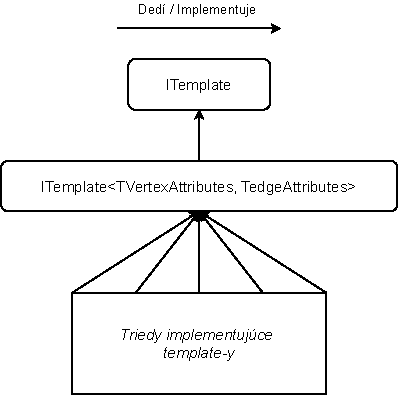
\includegraphics[]{img/templatey_architektura}
\caption{Diagram popisujúci objektovú štruktúru template-ov.} 
\label{obr05:templatey_architektura}
\end{figure}

\section{Mapy}

Táto oblasť sa stará o~vytváranie a~správu mapových objektov. Viac informácií o~koncepte Máp je možné nájsť v~Podsekcii~\ref{mapy}.

Hlavným uzlom pre~komunikáciu z~Model view vrstvy je singleton trieda \texttt{TemplateManager}. Tá ponúka kolekciu mapových formátov, ktorá obsahuje zástupcov všetkých mapových typov, ktoré~je možné v~aplikácii využiť. Každý zástupca zastupuje jeden typ mapy, jeden formát. Popri tom ponúka metódy pre~vytváranie mapových inštancií a~metódy pre~identifikáciu mapových formátov. 

V~následujúcich odsekoch popíšeme objektovú štruktúru máp a~ich~zástupcov. Grafické znázornenie tejto architektúry je možné nahliadnuť v~Diagrame~\ref{obr06:mapy_architektura}.   

\bigskip

Mapy sú reprezentované pomocou tried, ktoré~implementujú rozhranie \textbf{\texttt{IMap}}. Toto rozhranie nedefinuje žiadnu zaujímavú funkcionalitu. Obsahuje pár vlastností využívaných mimo vrstvy Model pre~identifikáciu mapy.

Triedy máp následne môžu implementovať niektoré z~ďalších definovaných rozhraní, ktoré~pridávajú svoje kontrakty. Tieto kontrakty sú zamerané na~geografické lokalizovanie a~rozlohu máp. Sú využívané predovšetkým pri~získavaní dodatočných výškových dát odpovedajúcich konkrétnej mape. Ak si je mapový typ vedomí toho, že~na~vytvorenie jeho mapovej reprezentácie bude potrebná výpomoc výškových dát, mal by implementovať aspoň jeden z~interface-ov, ktorý~definuje informácie o~geo-lokalite a~rozlohe mapy.

Ako už bolo naznačené, pri~mapách je potrebné, aby~v~aplikácii niekto zastupoval ich formáty. K~tomuto slúžia triedy implementujúce trojicu rozhraní:
\begin{itemize}
    \item \textbf{\texttt{IMapFormat<out TMap>}} - Je určený pre~komunikáciu mimo vrstvy Model. Definuje vlastnosti, ktoré~sú potrebné pri~práci s~mapovým zástupcom vo~vonkajšom prostredí a~metódu na~vytváranie mapy zastupovaného typu. Tento interface by nemal byť priamo implementovaný.
    \item \textbf{\texttt{IMapIdentifier<in TMap>}} - Slúži na~identifikáciu odpovedajúceho mapového formátu pre~konkrétny typ mapy. Vďaka kontravariantnej povahe jeho typového parametru bude táto identifikácia fungovať správne aj~pre~potomkov typu \texttt{TMap}. Tento interface by nemal byť priamo implementovaný.
    \item \textbf{\texttt{IMapRepresentative<TMap>}} - Zastupuje jeden konkrétny typ/formát mapy. Je potomkom predošlých dvoch interface-ov - spája ich funkcionality. Tento interface je určený k~tomu, aby~bol priamo implementovaný mapovými zástupcami.   
\end{itemize}
Na to, aby~bolo možné mapový typ využiť v~aplikácii, musí byť jeho zástupca zahrnutý v~príslušnej kolekcii v~triede \texttt{MapManager}. Z~tohto dôvodu je na~mieste, aby~títo zástupcovia boli implementovaný ako singleton triedy.

Mapy podporujú návrhový vzor \textit{Generic visitor pattern}. Ten je definovaný ako pre~rozhranie \texttt{IMap}, tak aj~pre~rozhranie \texttt{IGeoLocatedMap} (pridáva kontrakt o~geografickej lokalite mapy).

\begin{figure}[h]\centering
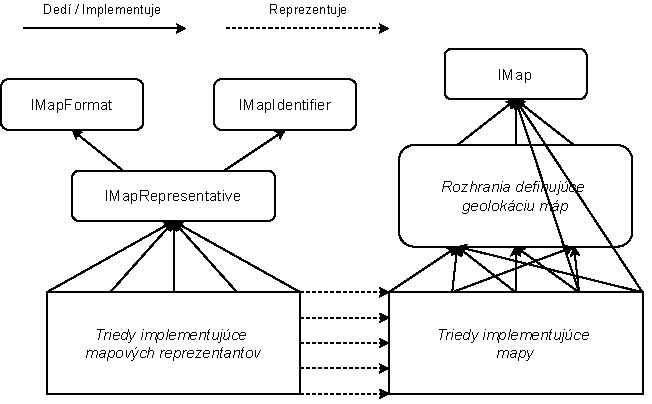
\includegraphics[]{img/mapy_architektura}
\caption{Diagram popisujúci objektovú štruktúru máp a ich zástupcov.} 
\label{obr06:mapy_architektura}
\end{figure}

\section{Mapové reprezentácie}

Ďalšia z~oblastí sa stará o~vytváranie a~spravovanie mapových reprezentácii/grafov. Čo do~obsahu aj~komplexnosti sa jedná o~jednu z~najväčších oblastí. Viac informácií o~koncepte mapových reprezentácií je možné nájsť v~Podsekcii~\ref{mapove_reprezentacie}.

Hlavným uzlom pre~prácu s~touto oblasťou z~vonkajšieho prostredia je singleton trieda \texttt{MapRepreManager}. Ten ponúka kolekciu obsahujúcu zástupcov všetkých typov mapových reprezentácií, ktoré~je možné v~aplikácii využiť. Popri tom obsahuje metódy určené na~
\begin{itemize}
    \item vytváranie mapových reprezentácií,
    \item identifikáciu reprezentácií vytvoriteľných pre~konkrétnu kombináciu typov template-u a~mapy,
    \item detekciu potreby výškových dát pri~konštrukcii mapovej reprezentácie.
\end{itemize}

V~následujúcich odsekoch popíšeme objektovú štruktúru mapových reprezentácií/grafov, ich implementácií a~zástupcov. Pre~jednoduchšie porozumenie je možné v~Diagrame~\ref{obr07:mapove_reprezentacie_architektura} nahliadnuť grafické znázornenie tejto architektúry. 

\bigskip

Štruktúra dát, ktoré~súvisia s~mapovými reprezentáciami odzrkadluje dvojakosť významov mapovej reprezentácie a~grafu ako bolo popísané v~Podsekcii~\ref{mapove_reprezentacie}. Každému typu mapovej reprezentácie je prisúdený konkrétny typ grafu.

Mapové reprezentácie/grafy sú v~aplikácii reprezentované triedami, ktoré~implementujú rozhranie \textbf{\texttt{IGraph<TVertexAttributes, TEdgeAttributes>}}. Toto rozhranie reprezentuje myšlienku grafu, ktorý~zastupuje konkrétnu mapovú reprezentáciu. Jeho typové parametre definujú atribúty, ktoré~sú používané v~jeho vrcholoch a~hranách. Obsahuje kontrakty, ktoré~musia grafy všetkých typov naplňovať. Aktuálne je to len jedna metóda vracajúca graf do~jeho základného stavu.

\texttt{IGraph<TVertexAttributes, TEdgeAttributes>} má za~predchodcu rozhranie \textbf{\texttt{IMapRepre}} reprezentujúce myšlienku samotnej mapovej reprezentácie. Cez toto rozhranie sú mapové reprezentácie/grafy distribuované vonkajšiemu svetu. K~tomuto účelu rozhranie definuje vlastnosti využívané mimo vrstvy Model. Grafová podstata mapových reprezentácií je tým vonkajšiemu svetu ukrytá a~len špecifické oblasti Model vrstvy ju znova nadobúdajú a~využívajú.

Každá mapová reprezentácia/graf má množinu svojich implementácií. Implementácie sú tvorené pre~konkrétne kombinácie template-ov a~mapových formátov. Konkrétny typ mapovej reprezentácie môže byť vytvorený len pre~takú kombináciu template-u a~mapového formátu, pre~ktorý je vytvorená príslušná implementácia.

V~aplikácii sú naďalej prítomné ďalšie rozhrania, ktoré~môžu (a mali by v~čo najväčšom rozsahu) jednotlivé grafy implementovať. Tieto rozhrania definujú kontrakty týkajúce sa vlastností a~funkcií generovaných grafov.

\bigskip

Na to aby~mohla byť mapová reprezentácia, graf či~implementácia v~aplikácii použitá, musí pre~ne existovať vhodný zástupca. Tento zástupca je následne poskytnutý na~patričnom mieste.
\begin{itemize}
    \item Zástupcovia typov mapových reprezentácií sú v aplikácii reprezentovaní triedami, ktoré~implementujú rozhranie \textbf{\texttt{IMapRepreRepresentative<out TMapRepre>}}. Tieto triedy sú určené (podobne ako typy mapových reprezentácií) pre~komunikáciu mimo vrstvy Model. Definujú vlastnosti, ktoré~sú využívané vonkajším svetom pre~získanie informácií o~zastupovanej mapovej reprezentácii. 
    
    Taktiež si držia indikátorovú kolekciu zástupcov všetkých implementácií zastupovanej mapovej reprezentácie. Táto kolekcia sa následne využíva pri~identifikácii použiteľných kombinácií template-ov a~mapových formátov a~pri samotnom vytváraní mapových reprezentácií/grafov.
    
    Nakoľko typ mapovej reprezentácia je vždy asociovaný s~nejakým typom grafu, zástupca typu mapovej reprezentácia disponuje aj~referenciou na~zástupcu typu daného grafu. Tento zástupca sa následne využíva v~procese vytvárania mapovej reprezentácie/grafu. Taktiež špecifické oblasti vrstvy Model ho môžu využiť k~otestovaniu vlastností zastupovaného grafu.

    Taktiež toto rozhranie definuje metódy pre~vytváranie zastupovaného typu mapovej reprezentácie. 

    Na~to, aby~bolo možné typ mapovej reprezentácie/grafu využiť v~aplikácii, musí byť jeho zástupca zahrnutý v~príslušnej kolekcii manažéra mapových reprezentácií.

    \item Zástupcovia grafových typov sú reprezentovaní triedami, ktoré~implementujú rozhranie \textbf{\texttt{IGraphRepresentative < out TGraph, TVertexAttributes, TEdgeAttributes>}}. Typové parametre definujú typ zastupovaného grafu a~typy atribútov, ktoré~sú použité v~jeho vrcholoch a~hranách. Tento interface nedefinuje žiadny kontrakt pre~grafových zástupcov. Implementuje iba metódy, ktoré~sú využívané v~procese vytvárania mapovej reprezentácie/grafu. Je využívaný špecifickými oblasťami vrstvy Model k~otestovaniu vlastností zastupovaného grafu.

    Každý zástupca grafu je asociovaný s~konkrétnym zástupcom mapovej reprezentácie. Ten si na~jeho inštanciu drží referenciu a~využíva ho v~procese vytvárania mapovej reprezentácie/grafu.

    \item Ku~reprezentácii zástupcov jednotlivých implementácií slúžia triedy, ktoré~dedia od abstraktnej triedy \textbf{\texttt{ElevDataIndepImplementationRep}} alebo~od abstraktnej triedy \textbf{\texttt{ElevDataDepImplementationRep}}. Tieto rozhrania disponujú dvojitou funkcionalitou:
    \begin{itemize}
        \item Obsahujú vlastnosti indikujúce template a~mapový formát, na~základe ktorých je implementácia mapovej reprezentácie/grafu agregovaná. Tieto vlastnosti sú naplnením kontraktu definovaného ich predchodcom \textbf{\texttt{IImplementationIndicator}}.
        \item Je schopná skonštruovať (alebo~nechať skonštruovať) zastúpenú implementáciu mapovej reprezentácie. Tieto triedy sa líšia predovšetkým v~potrebe dodatočných výškových dát v~procese tvorby danej implementácie. Schopnosť skonštruovať danú implementáciu je naplnením kontraktu jedného z~rozhraní \textbf{\texttt{IImplementationElevDataIndepConstr}}, respektíve \textbf{\texttt{IImplementationElevDataDepConstr}}. 
    \end{itemize}
    Taktiež disponujú množinou typových parametrov, z~ktorých každý má svoj špecifický význam:
    \begin{itemize}
        \item \texttt{TTemplate} - definuje typ template-u, pre~ktorý je zastupovaná implementácia vytvorená
        \item \texttt{TGraph} - definuje typ mapovej reprezentácie/grafu, pre~ktorý je zastupovaná implementácia vytvorená,
        \item \texttt{TVertexAttributes, TEdgeAttributes} - definujú typy atribútov použitých v~implementovanom grafe
        \item \texttt{TMap, TUsableSubMap} - tieto parametre sú jemne zavádzajúce. Prvý z~nich hovorí o~tom, aký typ mapy je navonok indikovaný pomocou vlastnosti mapového formátu. Druhý hovorí o~tom, ktorý~typ potomok typu \texttt{TMap} je v~skutočnosti potrebný na~vytvorenie mapovej reprezentácie. Malo by byť zaručené okolitým prostredím, že~pokiaľ je nejaká mapa správneho formátu, tak je určite možné ju použiť pre~vytvorenie mapovej reprezentácie. 
    \end{itemize}
    
    Zástupcovia jednotlivých implementácií mapovej reprezentácie sú zahrnutí v~kolekcii zástupcu tejto mapovej reprezentácie.

\end{itemize}

Bolo by vhodné, aby~všetci spomenutí zástupcovia boli implementovaní ako singleton triedy. Od každého z~nich je totiž za~celú dobu behu programu potrebné vytvoriť iba jedinú inštanciu, ktorá je poskytovaná zvyšku aplikácie na~patričnom mieste.

Poslednou súčasťou oblasti mapových reprezentácií sú triedy, ktoré~reprezentujú vrcholy a~hrany používané v~grafoch. Jednotlivé typy sa potom líšia dodávanými vlastnosťami.   

\begin{figure}[p]\centering
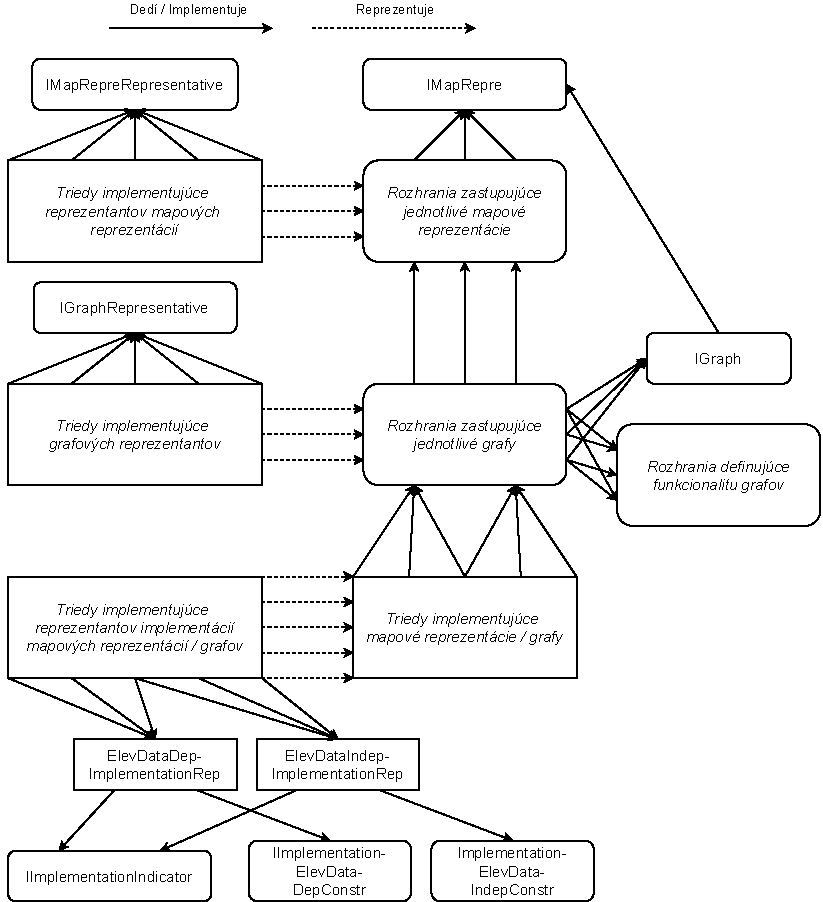
\includegraphics[]{img/mapove_reprezentacie_architektura}
\caption{Diagram popisujúci objektovú štruktúru mapových reprezentácií/grafov, ich implementácií a~zástupcov.} 
\label{obr07:mapove_reprezentacie_architektura}
\end{figure}

\pagebreak

\section{Užívateľské modely}

V~tejto oblasti sú vytvárané a~spravované užívateľské modely. Viac informácií o~koncepte užívateľských modelov je možné nájsť v~Podsekcii~\ref{uzivatelske_modely}.

Hlavným komunikačným uzlom s~touto oblasťou pre~Model view vrstvu je singleton trieda \texttt{UserModelManager}. Ten ponúka kolekciu všetkých typov užívateľských modelov, ktoré~je možné v~aplikácii využiť. Mimo to implementuje metódy pre:
\begin{itemize}
    \item Serializáciu a~deserializáciu užívateľských modelov do/z súborov.
    \item Vytváranie nových inštancií užívateľských modelov.
    \item Všeobecnú identifikáciu typov užívateľských modelov na~základe rôznych typov argumentov.
\end{itemize}

V~následujúcich odsekoch popíšeme objektovú štruktúru užívateľských modelov a~ich~zástupcov. Grafické znázornenie tejto architektúry je možné nahliadnuť v~Diagrame~\ref{obr08:uzivatelske_modely_architektura}.   

\bigskip

Užívateľské modely sú v~aplikácii reprezentované triedami, ktoré~implementujú rozhranie \textbf{\texttt{IUserModel<out TTemplate>}}.  Prostredníctvom tohto rozhrania sú užívateľské modely využívané mimo vrstvy Model. Z~tohto dôvodu definuje informatívne vlastnosti, ktoré~sú potrebné prevažne vo~vonkajšom svete. Popri tom definuje ešte aj~kontrakty zaručujúce schopnosť serializácie užívateľského modelu. Každý užívateľský model je viazaný na~konkrétny template-u, typu \texttt{TTemplate}. K~tomu si každý užívateľský model nesie aj~referenciu na~inštanciu daného template-u.

Na to aby~bol užívateľský model použiteľný vo~vyhľadávacích algoritmoch, nestačí aby~implementoval predchádzajúce základné rozhranie. Je potrebné aby~implementoval následnícke rozhranie \textbf{\texttt{IComputingUserModel<out TTemplate, in TVertexAttributes, in TEdgeAttributes>}}. Tento interface sám o~sebe nedefinuje žiadny kontrakt. Až jeho následníci definujú výpočtovú funkcionalitu, ktorú implementujúci užívateľský model vie ponúknuť napríklad vyhľadávaciemu algoritmu. 

Jedným z~týchto následníkov je interface \textbf{\texttt{IWeightComputingUserModel<out TTemplate, in TVertexAttributes, in TEdgeAttributes>}}. Toto rozhranie zaisťuje schopnosť užívateľského modelu, na~základe dodaných vrcholových a~hranových atribútov, vypočítať váhu odpovedajúcej hrany. Túto funkcionalitu by mali spĺňať všetky užívateľské modely, nakoľko veľká časť vyhľadávacích algoritmov potrebuje poznať váhu jednotlivých hrán pre~správny výber postupu.

Oproti výpočtovým rozhraniam existuje v~tejto oblasti aj~špecifické rozhranie \textbf{\texttt{ISettableUserModel}}. Toto rozhranie musia implementovať všetky typy užívateľských modelov, ktoré~sú určené na~to, aby~v~nich užívateľ mohol konfigurovať nastaviteľné hodnoty (tzv.\textit{Adjustables}) vzhľadom na~svoje preferencie. Kontrakt ktorý~definuje zaručuje dodanie kolekcie týchto nastaviteľných hodnôt, aby~mohli byť dodané užívateľovi a~ten s~nimi mohol pracovať. Mechanizmus vytvárania a~nastavovania užívateľských modelov zatiaľ v~aplikácii nie je implementovaný, a~teda toto rozhranie aktuálne čaká na~svoje využitie.  

\bigskip

V~aplikácii je potrebné, aby~existencia jednotlivých typov užívateľských modelov bola nejakým spôsobom zastúpená. Týmito zástupcami sú triedy implementujúce následujúcu trojicu rozhraní:
\begin{itemize}
    \item \textbf{\texttt{IUserModelType<out TUserModel, out TTemplate>}} - Je určený pre~komunikáciu mimo vrstvy Model. Definuje vlastnosti, ktoré~sú potrebné pri~práci so~zástupcom užívateľského modelu vo~vonkajšom prostredí. 
    
    Taktiež obsahuje referenciu na~template, na~ktorý je zastupovaný užívateľský model viazaný a~definuje metódy slúžiace na~deserializáciu a~vytváranie nových užívateľských modelov. Implementácie deserializácie zástupcu a~serializácie zastupovaného užívateľského modelu sa musia zhodovať. 
    
    Tento interface by nikdy nemal byť priamo implementovaný.
    \item \textbf{\texttt{IUserModelTemplateBond<in TTemplate>}} - Reprezentuje väzbu užívateľského modelu a~template-u.  Vďaka kontravariantnej povahe jeho template-ového typového parametru bude táto identifikácia fungovať správne aj~pre~prípadných potomkov typu \texttt{TTemplate}. Tento interface by nikdy nemal byť priamo implementovaný.
    \item \textbf{\texttt{IUserModelRepresentative<TUserModel,TTemplate>}} - Zastupuje jeden konkrétny typ užívateľského modelu viazaného na~jeden konkrétny typ template-u. Je potomkom predošlých dvoch interface-ov - spája ich funkcionality. Tento interface je určený k~tomu, aby~bol priamo implementovaný zástupcami užívateľských modelov.   
\end{itemize}

Na to, aby~bolo možné typ užívateľského modelu využiť v~aplikácii, musí byť jeho zástupca zahrnutý v~príslušnej kolekcii triedy \texttt{UserModelManager}. Z~tohto dôvodu je na~mieste, aby~títo zástupcovia boli implementovaný ako singleton-y.

\begin{figure}[h]\centering
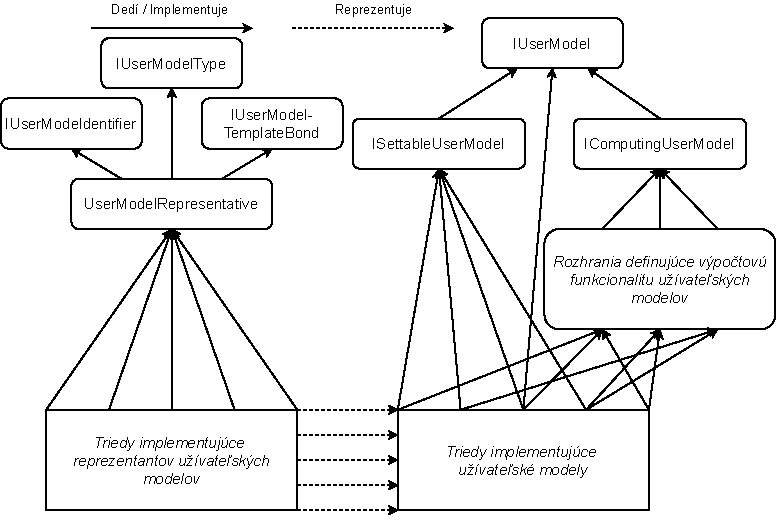
\includegraphics[]{img/uzivatelske_modely_architektura}
\caption{Diagram popisujúci objektovú štruktúru užívateľských modelov a~ich~zástupcov.} 
\label{obr08:uzivatelske_modely_architektura}
\end{figure}

\section{Vyhľadávacie algoritmy}

Táto oblasť zahrnuje mechanizmy spravujúce algoritmy pre~vyhľadávanie ciest v~mapových reprezentáciách. Viac informácií o~vyhľadávacích algoritmoch samotných je možné nájsť v~Podsekcii~\ref{vyhladavacie_algoritmy}. 

Hlavným komunikačným uzlom s~touto oblasťou pre~Model view vrstvu je singleton trieda \texttt{SearchingAlgorithmMan}. Táto trieda zverejňuje v~kolekcii všetky použiteľné vyhľadávacie algoritmy aplikácie. Popri tom obsahuje metódy zabezpečujúce: 
\begin{itemize}
    \item spúšťanie procesu vyhľadávania cesty na~základe dodaného užívateľského modelu a~mapovej reprezentácie
    \item dodávanie \textit{executor}-u vyhľadávacieho algoritmu
    \item identifikáciu vyhľadávacích algoritmov spustiteľných pre~konkrétne kombinácie mapových reprezentácií a~užívateľských modelov 
\end{itemize}

V~následujúcich odsekoch popíšeme objektovú štruktúru vyhľadávacích algoritmov a~ich~implementácií. Jednoduché grafické znázornenie tejto architektúry je možné nahliadnuť v~Diagrame~\ref{obr09:vyhladavacie_algoritmy_architektura}.   

\bigskip

Vyhľadávacie algoritmy sú v~aplikácii reprezentované pomocou tried, ktoré~implementujú rozhranie \textbf{\texttt{ISearchingAlgorithm}}. Každý algoritmus môže byť implementovaný niekoľkými spôsobmi. Rozhranie preto definuje kolekciu, v~ktorej by mali byť všetky použiteľné implementácie daného algoritmu zverejnené. Ďalej definuje a~zároveň implementuje metódy, ktoré~slúžia na:
\begin{itemize}
    \item testovanie, či~zástupcovia typov mapovej reprezentácie a~užívateľského modelu zastupujú použiteľnú kombináciu pre~daný algoritmus. Teda či~existuje implementácia algoritmu, pre~ktorú sú vlastnosti zastupovaných typov dostatočné na~použitie, 
    \item samotné spúšťanie vyhľadávacieho procesu. K~tomuto účelu sa vyberie pre~vstupné argumenty vhodná implementácia algoritmu,
    \item možnosť získania \textit{executor}-u daného algoritmu. Executor sa vytvorí na~základe vhodnej implementácie algoritmu.
\end{itemize}
Inštancia každého použiteľného vyhľadávacieho algoritmu musí byť obsiahnutá v~kolekcii vyhľadávacích algoritmov v~príslušnom manažérovi. Inak nebude aplikácia daný vyhľadávací algoritmus registrovať. 

Implementácie vyhľadávacích algoritmov sú reprezentované triedami, ktoré~implementujú rozhranie \textbf{\texttt{ISearchingAlgorithmImplementation}}. Toto rozhranie definuje podobné myšlienky funkcionalít tým z~rozhrania \texttt{ISearchingAlgorithm}: testovanie typov vstupných mapových reprezentácií a~užívateľských modelov, spúšťanie vyhľadávacieho procesu a~vytváranie svojich executor-ov. V~tomto prípade však nie je táto funkcionalita implementovaná rozhraním a~je potrebné aby~ju implementácie algoritmov doplnili sami. Na~to aby~implementácia algoritmu mohla byť použitá, musí byť obsiahnutá v~kolekcii implementácií odpovedajúceho vyhľadávacieho algoritmu. 

Výsledkom vyhľadávania je inštancia triedy, ktorá implementuje rozhranie \textbf{\texttt{IPath<out TVertexAttributes, out TEdgeAttributes>}}. Toto rozhranie reprezentuje nájdenú cestu algoritmom pričom môže v~sebe niesť atribúty typov \texttt{TVertexAttributes} a~\texttt{TEdgeAttributes}. Neskôr v~Model view vrstve je z~tejto cesty vytvorený report, ktorý~je následne vyššími vrstvami spracovaný a~predvedený užívateľovi. Pre~komunikáciu mimo Model vrstvy sa využíva jeho predchodca \texttt{IPath}. Toto rozhranie by nemalo byť nikdy priamo implementované. 

Vyhľadávacie algoritmy taktiež môžu počas svojho behu podávať report-y o~stave vyhľadávania prostredníctvom objektov tried, ktoré~implementujú rozhranie \textbf{\texttt{ISearchingState<out TVertexAttributes, out TEdgeAttributes>}}. Algoritmus nechá z~týchto stavov agregovať report a~podá ho k~následnému spracovaniu a~predvedeniu užívateľovi.

Obidve vyššie spomenuté rozhrania taktiež podporujú návrhový vzor \textit{generic visitor pattern}. 

Pokiaľ je po~algoritme požadované vytvorenie jeho executor-u, algoritmus zavolá vhodnú svoju implementáciu nech executor vytvorí. Tá ho inicializuje pomocou dodanej mapovej reprezentácie, užívateľského modelu a~pridá delegáta na~svoju špecifickú metódu zabezpečujúcu beh algoritmu pre~executor.

Všetky triedy reprezentujúce vyhľadávacie algoritmy a~ich implementácie by mali byť implementované ako singleton triedy. Ich inštancie budú totiž vytvorené v~aplikácii len jeden krát.


\begin{figure}[h]\centering
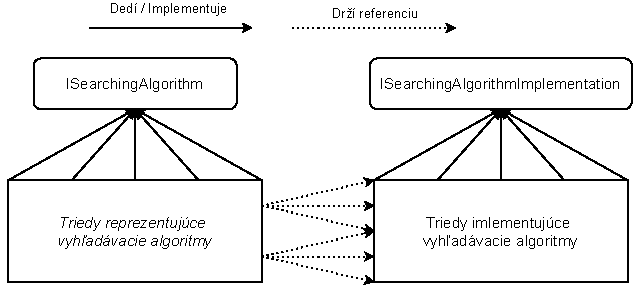
\includegraphics[]{img/vyhladavacie_algoritmy_architektura}
\caption{Diagram popisujúci objektovú štruktúru vyhľadávacích algoritmov a~ich~implementácií.} 
\label{obr09:vyhladavacie_algoritmy_architektura}
\end{figure}

\pagebreak

\section{Výškové dáta}

Oblasť pre~správu a~manipuláciu s~výškovými dátami. Viac informácií o~funkcii výškových dát v~aplikácii je možné nájsť v~Podsekcii~\ref{vyskove_data}. 

Hlavným komunikačným uzlom s~touto oblasťou z~vrstvy Model view je singleton trieda \texttt{ElevDataManager}. Tá ponúka kolekciu všetkých použiteľných zdrojov výškových dát v~aplikácii. Popri tom doručuje metódy pre~manipuláciu s~výškovými dátami (sťahovanie a~odstraňovanie) a~taktiež metódy, ktoré~testujú prítomnosť a~vracajú prítomné výškové dáta odpovedajúce rozlohe konkrétnej mapy.

V~následujúcich odsekoch popíšeme objektovú štruktúru výškových dát, ich zdrojov, distribúcií a~regiónov. Pre lepšie porozumenie je možné v~Diagrame~\ref{obr10:vyskove_data_architektura} nahliadnuť grafické znázornenie architektúry týchto štruktúr.   

\bigskip

Výškové dáta sú v~aplikácii reprezentované triedami, ktoré~implementujú rozhranie \textbf{\texttt{IElevData}}. Toto jednoduché rozhranie definuje metódy, ktoré~dokážu k~zadanej geografickej polohe vrátiť jej nadmorskú výšku. Inštancie týchto tried su na~mieru vytvárané tak, aby~dokázali dodať výškové dáta odpovedajúce polohe a~rozlohe konkrétnej mapy. 

Výškové dáta sú dodávané jednotlivými zdrojmi. Tie sú v~aplikácii reprezentované triedami, ktoré~implementujú rozhranie \textbf{\texttt{IElevDataSource}}. Zdroje výškových dát sú zložené z~viacerých distribúcií, ktoré~následne už dodávajú potrebnú funkcionalitu pre~prácu s~nimi spravovanými, výškovými dátami. Preto rozhranie \texttt{IElevDataSource} definuje kolekciu, v~ktorej by mali byť uložené všetky distribúcie daného zdroja na~to, aby~mohli byť v~aplikácii použité. Popri tom definuje ďalších pár vlastností, ktoré~sú využívané mimo vrstvy Model (napr. meno daného zdroja).

Jednotlivé distribúcie výškových dát sú v~aplikácii reprezentované triedami, ktoré~implementujú rozhranie \textbf{\texttt{IElevDataDistribution}}. Každá z~týchto tried je zodpovedné za~prácu s~konkrétnou distribúciou výškových dát. Zabezpečujú sťahovanie, odstraňovanie a~informovanie o~ich prítomnosti. Je ponechané na~zodpovednosti implementácií, akým spôsobom budú dáta ukladané, načítané do~pamäte a~spracovávané do~inštancií implementácií rozhrania \texttt{IElevData}.

Rozhranie \texttt{IElevDataDistribution} by nemalo byť implementované priamo. Namiesto toho by mali byť implementované rozširujúce rozhrania \textbf{\texttt{ICredentials-} \texttt{NotRequiringElevDataDistribution}} a~\textbf{\texttt{ ICredentialsRequiringElevData- } \texttt{Distribution}},  ktoré~pridávajú samotnú metódu umožňujúcu sťahovanie výškových dát. Tieto metódy, resp. rozhrania, sa líšia v~potrebe autorizácie pri~získavaní výškových dát zo~vzdialených zdrojov.  

Manipulovanie s~výškovými dátami prebieha po~takzvaných \textit{regiónoch}. Každá distribúcia si tvar a~veľkosť svojich regiónov určuje sama. Následne tieto regióny sprostredkováva v~kolekcii \texttt{AllTopRegions}, ktorá je definovaná rozhraním \texttt{IElevDataDistribution}.

Regióny sú reprezentované triedami, ktoré~dedia od abstraktnej triedy \textbf{\texttt{Region}} a~jej potomkov \textbf{\texttt{TopRegion}} a~\textbf{\texttt{SubRegion}}. Región ako taký definuje svoje meno, svoj tvar za~pomoci reťazca geografických súradníc a~množinu svojich pod-regiónov. Taktiež definuje identifikátor svojej prítomnosti. Teda toho, čí sú jemu odpovedajúce výškové dáta stiahnuté v~počítači a~pripravené na~použitie alebo~nie.

Tento indikátor by mal byť aktualizovaný vždy keď sa prítomnosť dát regiónu zmení. Dôležité však je, že~táto informácia by mala byť zachovaná naprieč behmi aplikácie. Teda ak sú v~jednom behu aplikácie stiahnuté výškové dáta pre~konkrétny región, v~následujúcom behu by mal región indikovať, že~sú jemu zodpovedajúce dáta stále k~dispozícii.

Regióny sú naďalej delené na~\textit{vrcholové regióny} a~\textit{pod-regióny}. Pod-regióny sú vždy viazané na~nejaký vyšší región a~reprezentujú nejakú jeho časť. Vrcholový región potom jednoducho nie je nikoho pod-regiónom. Spomínaná kolekcia \texttt{AllTopRegions} obsahuje práve vrcholové regióny definované danou distribúciou.    


\begin{figure}[h]\centering
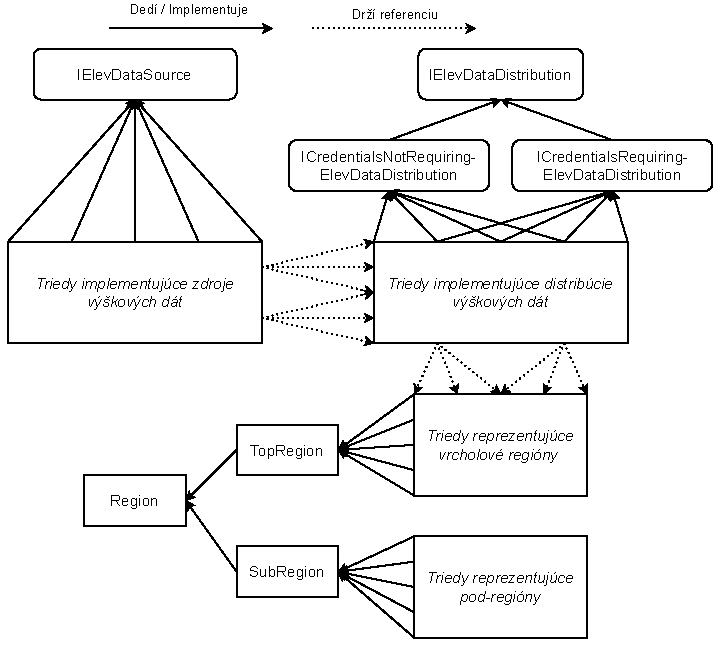
\includegraphics[]{img/vyskove_data_architektura}
\caption{Diagram popisujúci objektovú štruktúru zdrojov, distribúcií a~regiónov výškových dát.} 
\label{obr10:vyskove_data_architektura}
\end{figure}

\pagebreak

\section{Grafika}

Táto oblasť sa zaoberá problematikou vytvárania objektov, z~ktorých sa skladajú grafické reprezentácie rôznych dátových štruktúr. Agregácia grafických objektov sa vykonáva špecifickým asynchrónnym postupom. Vytvorené grafické objekty sa plnia do~tzv \textit{kolektoru}. Tým pádom je možné vytvorené objekty paralelne spracovávať a~zobrazovať ihneď po~ich vytvorení. 

Aplikácia obsahuje hneď dva hlavné uzly pre~komunikáciu s~touto oblasťou:
\begin{itemize}
    \item \texttt{GraphicsManager} je hlavným uzlom pre~komunikáciu prichádzajúcu z~Model view vrstvy. Zabezpečuje agregáciu grafických objektov pre~rôzne dátové štruktúry aplikácie ako sú napríklad mapy.
    \item \texttt{GraphicsSubManager} slúži k~rovnakému účelu ako \texttt{GraphicsManager}, avšak pre~komunikáciu priamo z~vrstvy Model. Reprezentuje prívetivejší spôsob komunikácie so~zachovaním typových informácií. Dátové štruktúry, pre~ktoré zabezpečuje táto trieda agregáciu grafiky, sú napríklad nájdené cesty a~stavy vyhľadávacích algoritmov. 
\end{itemize}
Obidve tieto triedy sa riadia návrhovým vzorom singleton.

\bigskip

Grafické objekty sú v~aplikácii reprezentované triedami, ktoré~implementujú rozhranie \textbf{\texttt{IGraphicObject}}.Toto rozhranie neimplementuje takmer žiadnu funkcionalitu okre podpory návrhového vzoru \textit{Generic visitor pattern}.

Aby bolo možné grafiku dodanej mapy, cesty či~stavu extrahovať, musí pre~ňu existovať trieda implementujúca rozhranie \textbf{\texttt{IGraphicsAggregator}}, teda presnejšie jedného z~jeho špecializovaných potomkov. Títo \textit{agregátori} následne dostanú objekt na~spracovanie a~kolektor, do~ktorého sa majú naklásť vytvorené grafické objekty.

V~prípade ciest a~stavov vyhľadávacieho algoritmu dostane agregátor aj~užívateľský model, ktorý~môže využiť na~výpočet niektorých hodnôt z~vrcholových a~hranových atribútov uložených v~dodaných cestách/stavoch. Je však potrebné zdôrazniť, že~užívateľský model možno nebude schopný tieto služby doručiť. V~takom prípad sa musí agregátor zaobísť bez nich. Je možnosť, aby~tieto vlastnosti vynucoval napríklad vyhľadávací algoritmus, ktorý~pozná potreby pre~extrahovanie grafiky ním používaného typu cesty či~stavu vyhľadávania.

Bolo by namieste, keby každý užívateľský model dokázal z~atribútov vyťažiť aspoň pozície vrcholov mapovej reprezentácie, aby~bolo možné nakresliť aspoň základnú reprezentáciu nájdenej cesty či~stavu. 

\bigskip

Nakoniec sú v~tejto oblasti definované dve rozhrania ktoré~slúžia pre~reprezentáciu grafického zdroja. \textbf{\texttt{IGraphicsSource}} definuje jedinú vlastnosť a~to zdrojovú kolekciu grafických objektov. Táto zdrojová kolekcia je typu \texttt{SourceList} patriaceho do~framework-u \textit{Reactive UI}. vo~vyšších vrstvách MVVM(MV) architektúry je následne možné tento zdrojový zoznam sledovať a~reagovať na~jeho aktualizácie. 

Špecializácia predošlého rozhrania \textbf{\texttt{IGroundGraphicsSource}} dodáva ešte nutnosť, aby~daný grafický zdroj definoval aj~svoju rozlohu. Triedy implementujúce toto rozhranie sú často využívané ako akési základné grafiky, ktorých rozlohe sa ostatné grafické zdroje prispôsobujú.

Implementácie týchto rozhraní sú väčšinou vytvárané mimo vrstvy Model. Sú na~mieru vytvorené pre~konkrétnu aplikačnú logiku. 

\section{Reportovanie}

Oblasti spravujúcej grafiku je architektúrou veľmi podobná oblasť vytvárajúca report-y na~základe rôznych typov dátových štruktúr. V~aktuálnej podobe aplikácie sú týmito štruktúrami cesty, nájdené vyhľadávacími algoritmami a~stavy vyhľadávacích algoritmov. Táto oblasť veľmi často využíva služby triedy \texttt{GraphicsSubManager} pre~získavanie grafiky, ktorá je pridaná do~obsahu report-ov.

Oblasť obsahuje opäť dva hlavné komunikačné uzly:
\begin{itemize}
    \item \texttt{ReportManager} je hlavným uzlom pre~komunikáciu prichádzajúcu z~Model view vrstvy. Aktuálne zabezpečuje vytváranie report-ov pre~nájdené cesty vyhľadávacím algoritmom.
    \item \texttt{ReportSubManager} slúži k~rovnakému účelu ako \texttt{ReportManager}, avšak pre~komunikáciu priamo z~vrstvy Model. Reprezentuje prívetivejší spôsob komunikácie so~zachovaním typovej informácie. Aktuálne zabezpečuje vytváranie report-ov pre~nájdené cesty a~stavy vyhľadávaní.
\end{itemize}
Obidve tieto triedy sa riadia návrhovým vzorom singleton.

\bigskip

Pre cesty a~stavy vyhľadávania sú reporty v~aplikácii reprezentované triedami, ktoré~implementujú rozhrania \textbf{\texttt{IPathReport}} a~\textbf{\texttt{ISearchingReport}}. Tieto rozhrania nedefinujú takmer žiadnu funkcionalitu, okrem podpory návrhového vzoru \textit{generic visitor pattern}.

Podobne ako v~oblasti spravujúcej grafiku, na~to, aby~pre~konkrétny typ dátovej štruktúry mohol byť report vytvorený, musí preňho existovať vhodná trieda implementujúca rozhranie \textbf{\texttt{IReportAggregator}}, resp. jedného z~jeho špecializovaných potomkov. Títo \textit{agregátori} následne dostanú dátovú štruktúru na~spracovanie a~v~niektorých prípadoch aj~užívateľský model, ktorý~môžu využiť na~výpočet hodnôt z~vrcholových a~hranových atribútov uložených v~dodaných dátach. Podobne však ako u grafických agregátorov, nie je zaručené, že~užívateľský model bude schopný požadované služby doručiť. 

\section{Parametre}

Posledná, jednoduchšia ale~o~to dôležitejšia oblasť je využívaná na~spravovanie a~ukladanie všemožných parametrov aplikácie. Hlavným uzlom pre~komunikáciu s~touto oblasťou je singleton trieda \texttt{ParamsManager}. V~tejto triede je možné uložiť od každého typu parametrov práve jednu inštanciu. Táto inštancia môže byť počas behu algoritmu rôzne upravovaná. Inštancie parametrov sú uložené v~slovníku pod kľúčom reprezentujúcom ich vlastný typ.  

Keď je zavolaná metóda \texttt{SaveAllParams}, tak sa trieda \texttt{ParamsManager} pokúsi všetky uložené parametre v~slovníku serializovať do~súborov pre~možnosť ich použitia v~budúcich behoch aplikácie.

Pri následnom behu aplikácie sú parametre deserializované zo~súborov tzv. \uv{lenivým} spôsobom. Keď je požiadané o~parametre typu, ktorý~v~slovníku nie je zastúpený, trieda sa pokúsi najprv zistiť, či~preňho neexistuje odpovedajúca serializácia. Ak áno, deserializuje sa inštancia odpovedajúcich parametrov, vloží sa do~slovníku a~vráti užívateľovi. Pokiaľ nie, poznačí sa do~slovníku neexistencia parametru daného typu a~navráti sa hodnota \texttt{null}.  

Serializácia a~deserializácia parametrov do~súborov, v~ktorých prežívajú beh aplikácie, prebieha za~pomoci singleton triedy \textbf{\texttt{DataSerializer}}. Táto trieda serializuje objekty do~súborov pomocou systémovej triedy \textit{\texttt{JsonSerializer}}. Súbory sú pomenované podľa typu daného serializovaného objektu. To znamená, že~v~jednu chvíli pre~každý dátový typ dokáže táto trieda serializovať jednu jedinú inštanciu. Pri~deserializácii, na~základe vstupného generického typového parametru nájde súbor s~odpovedajúcim menom a~pokúsi sa ho deserializovať do~inštancie daného typu.


  